\section{Experiment}\label{app:experiment}

This section presents all additional figures of \Cref{cha:experiment}.

\begin{figure}[!ht]
    \begin{subfigure}[b]{0.5\textwidth}%
    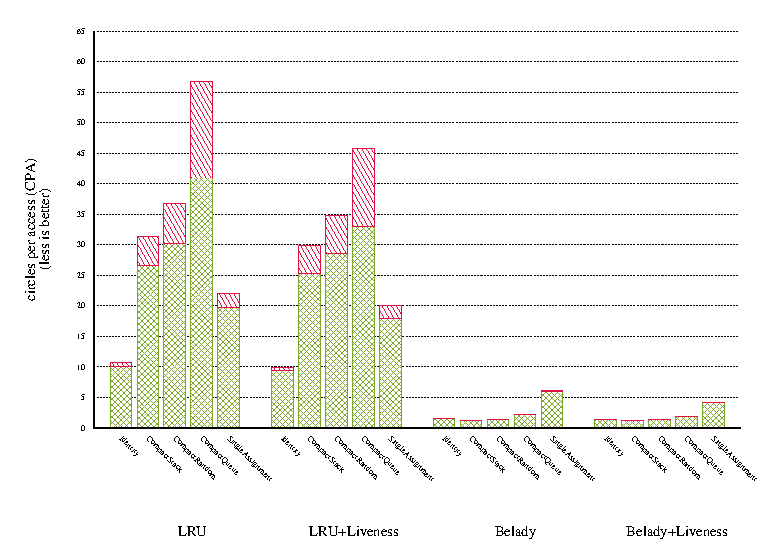
\includegraphics[width=\textwidth]{figs/plots/perf-misses-450-soplex.eps}
    \subcaption{Cache misses and cache hits}
  \end{subfigure}%
  \begin{subfigure}[b]{0.5\textwidth}%
    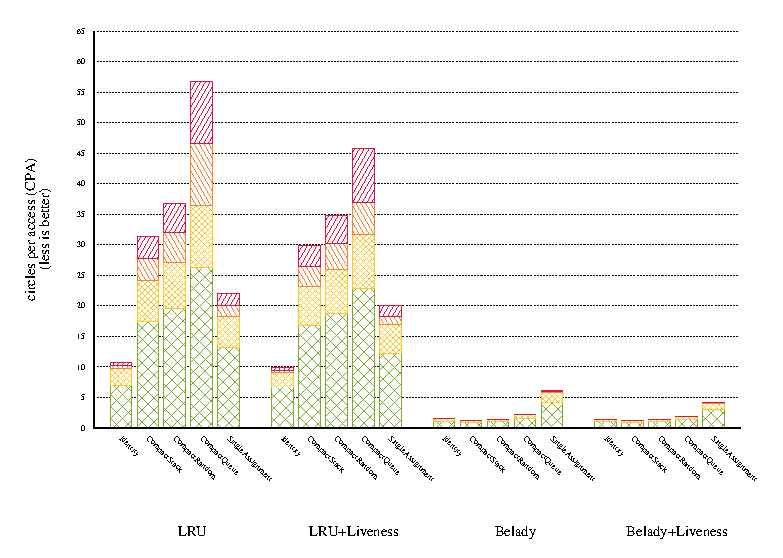
\includegraphics[width=\textwidth]{figs/plots/perf-450-soplex.eps}
    \subcaption{Types of memory operations}
  \end{subfigure}%
  \caption{Performance: 450.soplex}
  \label{fig:performance-450-soplex}
\end{figure}

\begin{figure}[!ht]
    \begin{subfigure}[b]{0.5\textwidth}%
    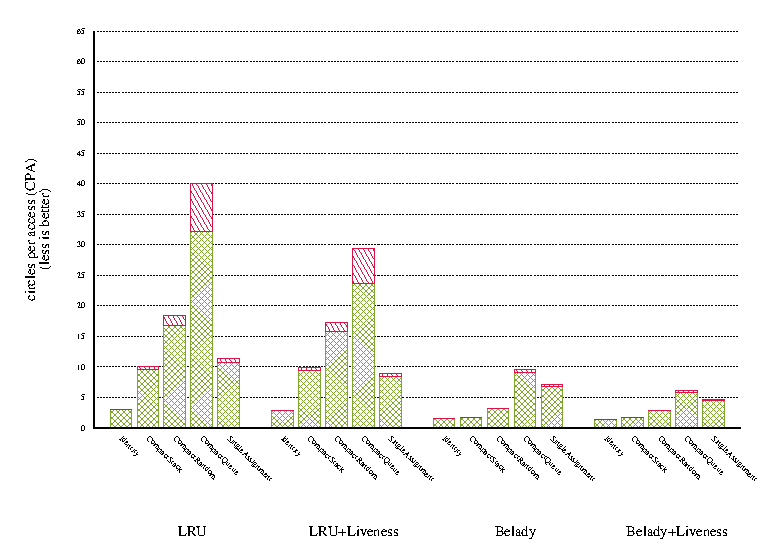
\includegraphics[width=\textwidth]{figs/plots/perf-misses-454-calculix.eps}
    \subcaption{Cache misses and cache hits}
  \end{subfigure}%
  \begin{subfigure}[b]{0.5\textwidth}%
    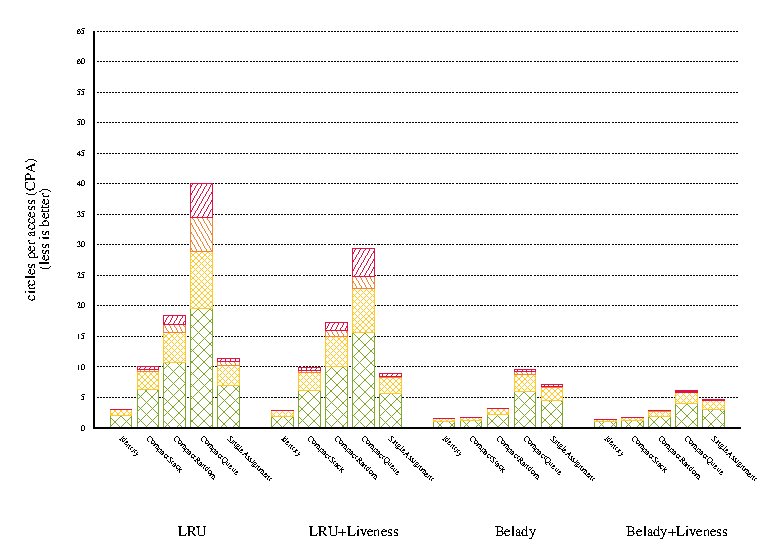
\includegraphics[width=\textwidth]{figs/plots/perf-454-calculix.eps}
    \subcaption{Types of memory operations}
  \end{subfigure}%
  \caption{Performance: 454.calculix}
  \label{fig:performance-454-calculix}
\end{figure}

\begin{figure}[!ht]
  \begin{subfigure}[b]{0.5\textwidth}%
    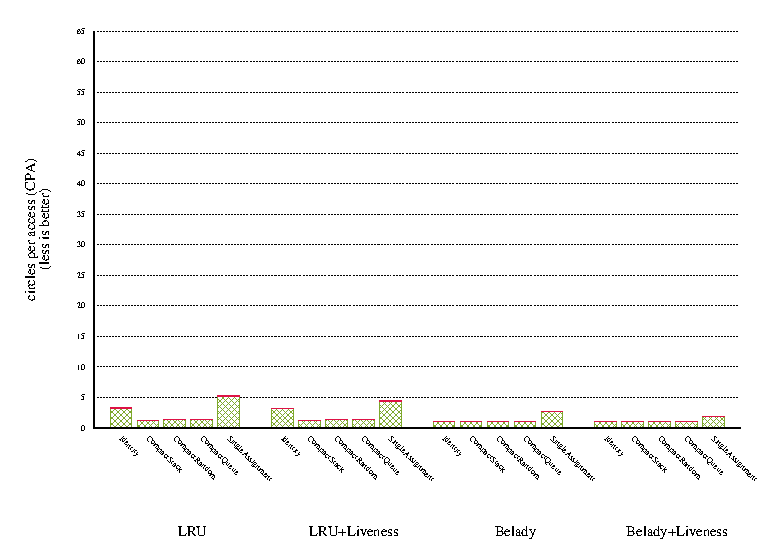
\includegraphics[width=\textwidth]{figs/plots/perf-misses-462-libquantum.eps}
    \subcaption{Cache misses and cache hits}
  \end{subfigure}%
  \begin{subfigure}[b]{0.5\textwidth}%
    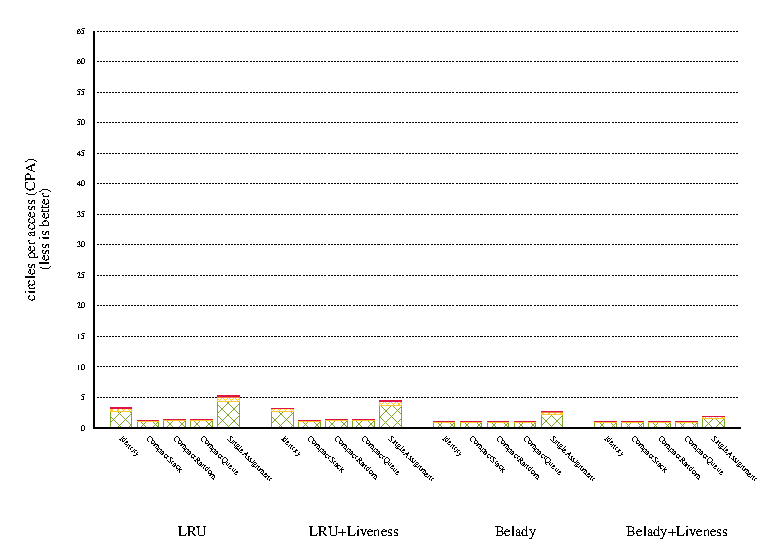
\includegraphics[width=\textwidth]{figs/plots/perf-462-libquantum.eps}
    \subcaption{Types of memory operations}
  \end{subfigure}%
  \caption{Performance: 462.libquantum}
  \label{fig:performance-462-libquantum}
\end{figure}

\begin{figure}[!ht]
  \begin{subfigure}[b]{0.5\textwidth}%
    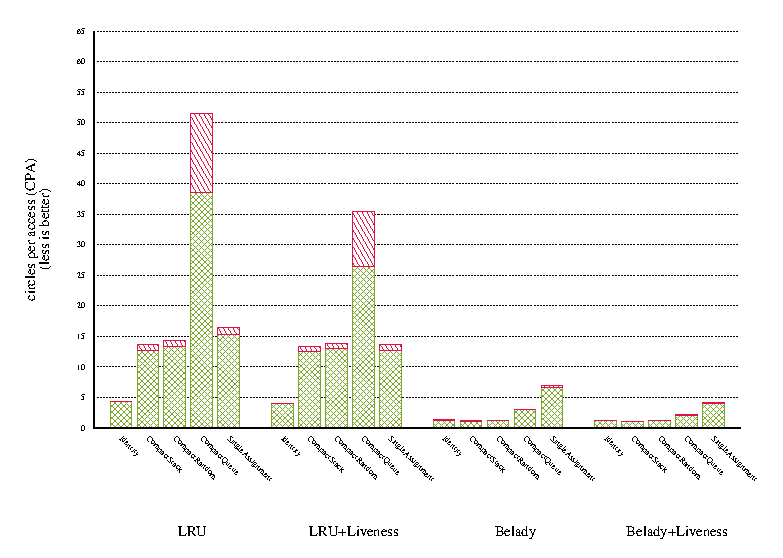
\includegraphics[width=\textwidth]{figs/plots/perf-misses-deltablue.eps}
    \subcaption{Cache misses and cache hits}
  \end{subfigure}%
  \begin{subfigure}[b]{0.5\textwidth}%
    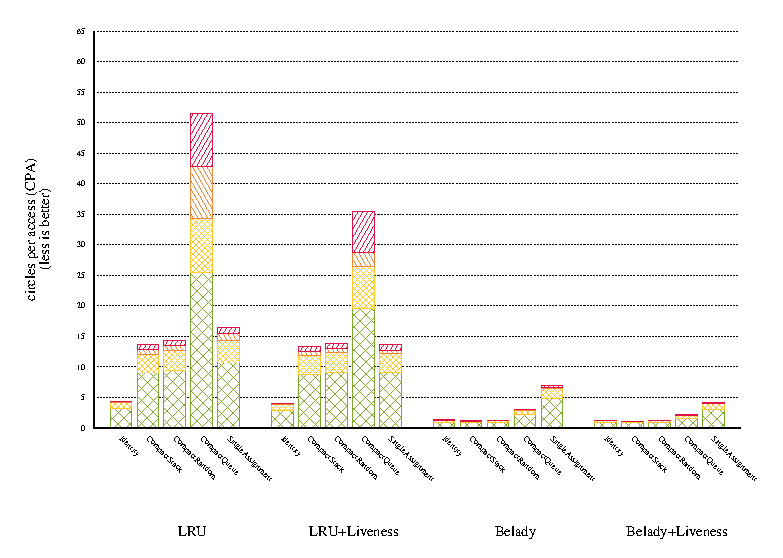
\includegraphics[width=\textwidth]{figs/plots/perf-deltablue.eps}
    \subcaption{Types of memory operations}
  \end{subfigure}%
  \caption{Performance: deltablue}
  \label{fig:performance-deltablue}
\end{figure}

\begin{figure}[!ht]
  \begin{subfigure}[b]{0.5\textwidth}%
    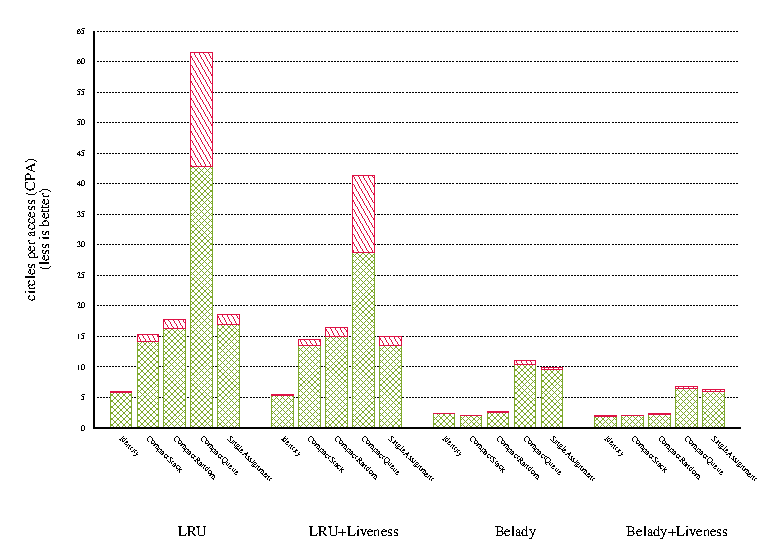
\includegraphics[width=\textwidth]{figs/plots/perf-misses-raytrace.eps}
    \subcaption{Cache misses and cache hits}
  \end{subfigure}%
  \begin{subfigure}[b]{0.5\textwidth}%
    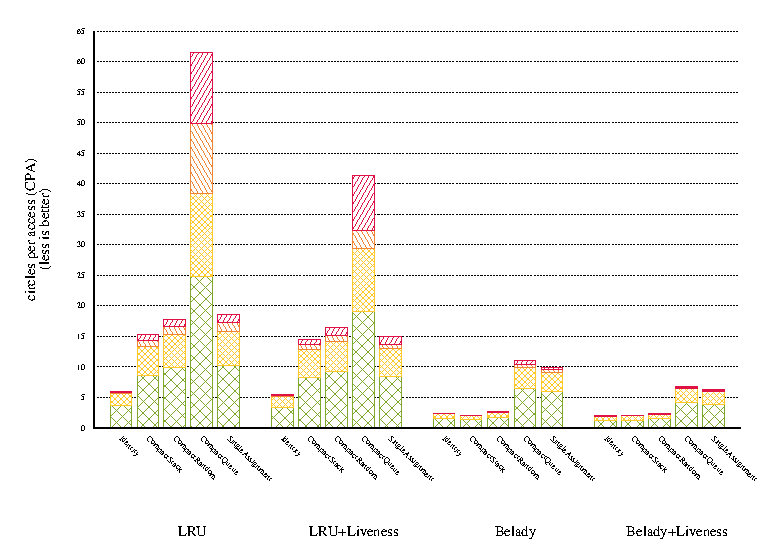
\includegraphics[width=\textwidth]{figs/plots/perf-raytrace.eps}
    \subcaption{Types of memory operations}
  \end{subfigure}%
  \caption{Performance: raytrace}
  \label{fig:performance-raytrace}
\end{figure}

\begin{figure}[!ht]
  \begin{subfigure}[b]{0.5\textwidth}%
    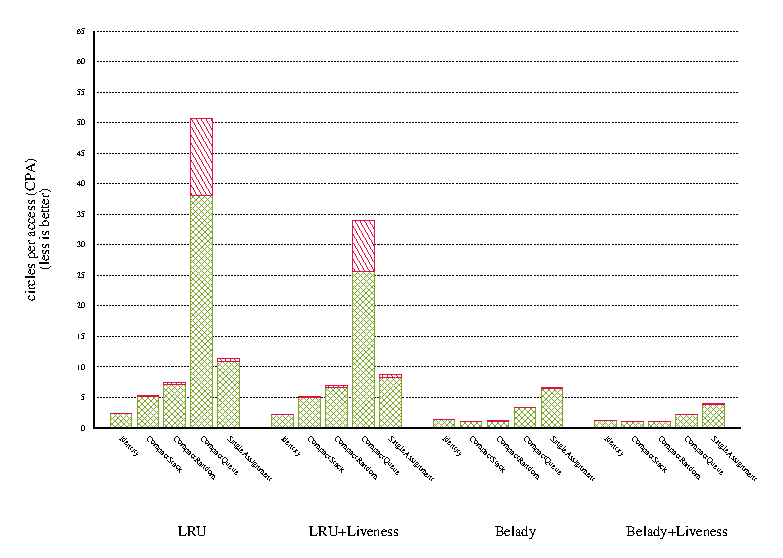
\includegraphics[width=\textwidth]{figs/plots/perf-misses-richards.eps}
    \subcaption{Cache misses and cache hits}
  \end{subfigure}%
  \begin{subfigure}[b]{0.5\textwidth}%
    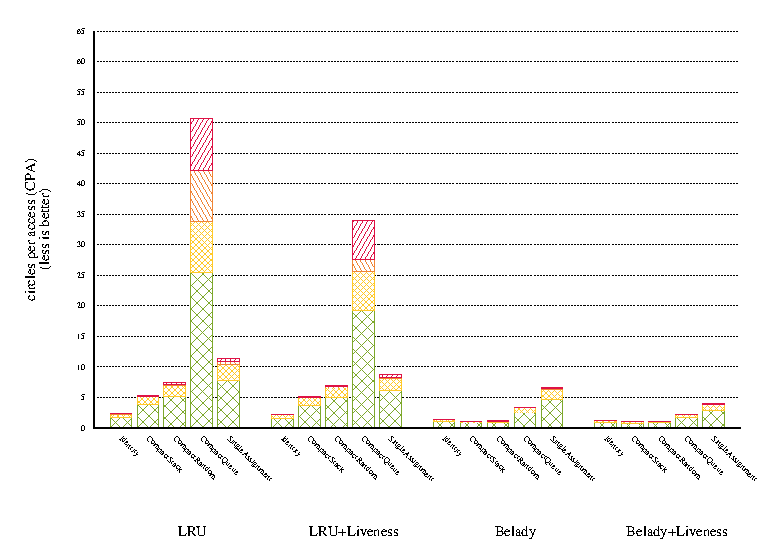
\includegraphics[width=\textwidth]{figs/plots/perf-richards.eps}
    \subcaption{Types of memory operations}
  \end{subfigure}%
  \caption{Performance: richards}
  \label{fig:performance-richards}
\end{figure}

\begin{figure}[!ht]
  \begin{subfigure}[b]{0.5\textwidth}%
    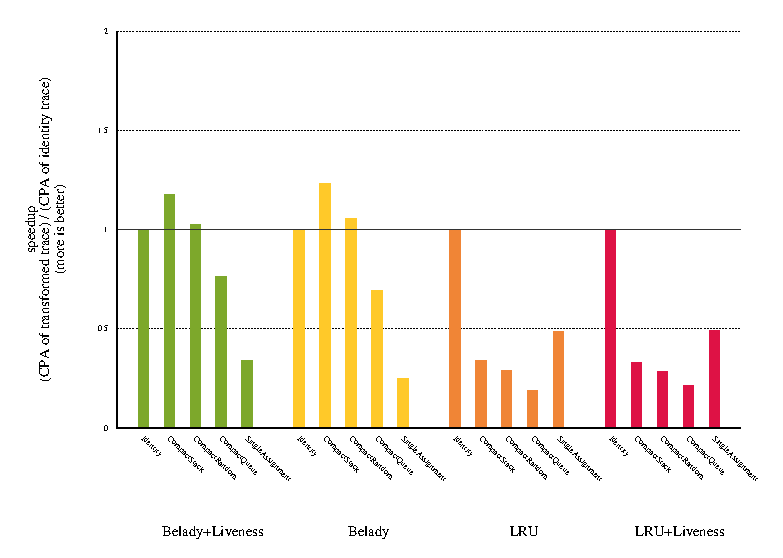
\includegraphics[width=\textwidth]{figs/plots/speedup-450-soplex.eps}
    \subcaption{Speedup}
  \end{subfigure}%
  \begin{subfigure}[b]{0.5\textwidth}%
    \includegraphics[width=\textwidth]{figs/plots/compaction-450-soplex.eps}
    \subcaption{Compaction}
  \end{subfigure}%
    \caption{Speedup \& Compaction: 450.soplex}
  \label{fig:speedup-compaction-450-soplex}
\end{figure}

\begin{figure}[!ht]
  \begin{subfigure}[b]{0.5\textwidth}%
    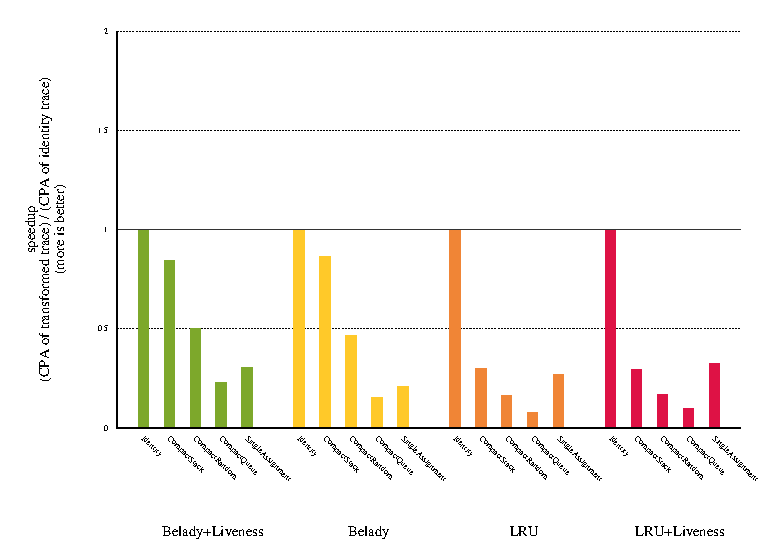
\includegraphics[width=\textwidth]{figs/plots/speedup-454-calculix.eps}
    \subcaption{Speedup}
  \end{subfigure}%
  \begin{subfigure}[b]{0.5\textwidth}%
    \includegraphics[width=\textwidth]{figs/plots/compaction-454-calculix.eps}
    \subcaption{Compaction}
  \end{subfigure}%
    \caption{Speedup \& Compaction: 454.calculix}
  \label{fig:speedup-compaction-454-calculix}
\end{figure}

\begin{figure}[!ht]
  \begin{subfigure}[b]{0.5\textwidth}%
    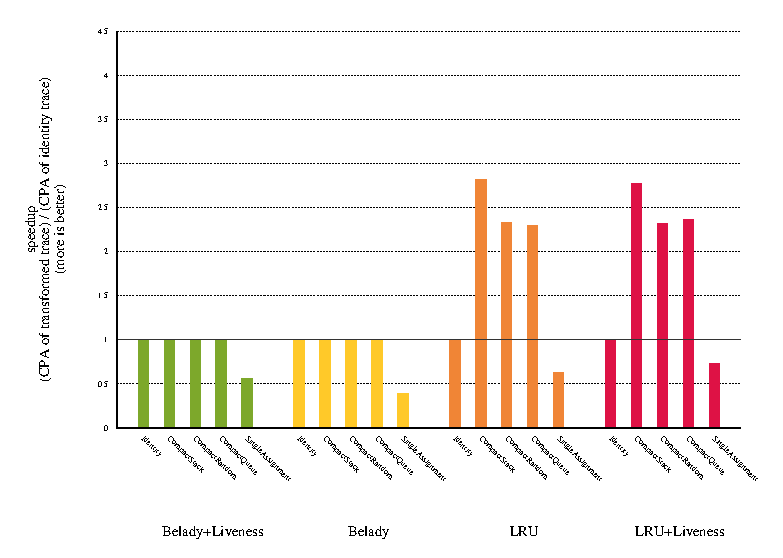
\includegraphics[width=\textwidth]{figs/plots/speedup-462-libquantum.eps}
    \subcaption{Speedup}
  \end{subfigure}%
  \begin{subfigure}[b]{0.5\textwidth}%
    \includegraphics[width=\textwidth]{figs/plots/compaction-462-libquantum.eps}
    \subcaption{Compaction}
  \end{subfigure}%
    \caption{Speedup \& Compaction: 462.libquantum}
  \label{fig:speedup-compaction-462-libquantum}
\end{figure}

\begin{figure}[!ht]
  \begin{subfigure}[b]{0.5\textwidth}%
    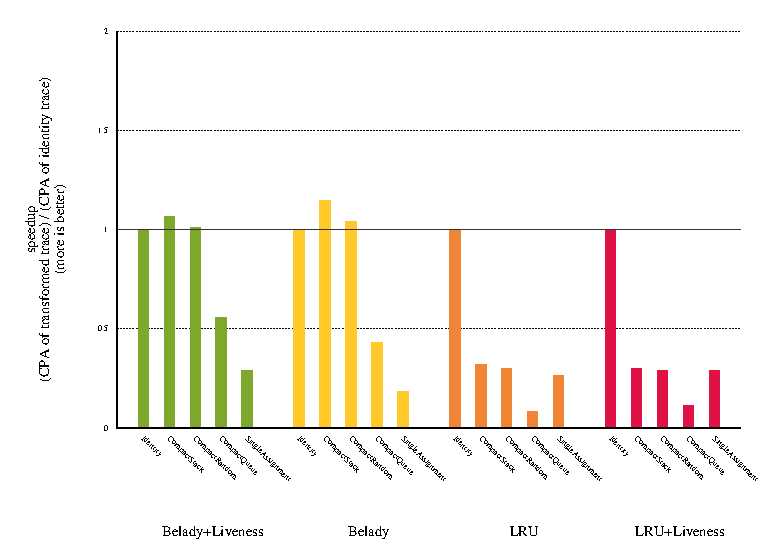
\includegraphics[width=\textwidth]{figs/plots/speedup-deltablue.eps}
    \subcaption{Speedup}
  \end{subfigure}%
  \begin{subfigure}[b]{0.5\textwidth}%
    \includegraphics[width=\textwidth]{figs/plots/compaction-deltablue.eps}
    \subcaption{Compaction}
  \end{subfigure}%
    \caption{Speedup \& Compaction: deltablue}
  \label{fig:speedup-compaction-deltablue}
\end{figure}

\begin{figure}[!ht]
  \begin{subfigure}[b]{0.5\textwidth}%
    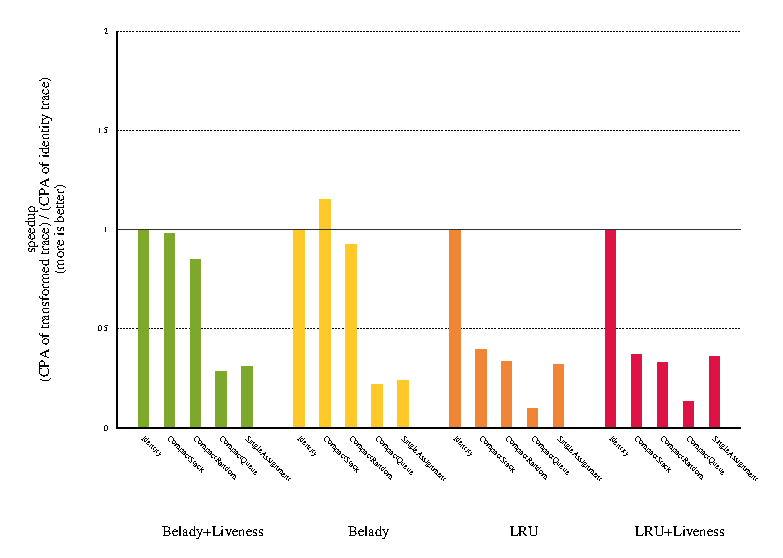
\includegraphics[width=\textwidth]{figs/plots/speedup-raytrace.eps}
    \subcaption{Speedup}
  \end{subfigure}%
  \begin{subfigure}[b]{0.5\textwidth}%
    \includegraphics[width=\textwidth]{figs/plots/compaction-raytrace.eps}
    \subcaption{Compaction}
  \end{subfigure}%
    \caption{Speedup \& Compaction: raytrace}
  \label{fig:speedup-compaction-raytrace}
\end{figure}

\begin{figure}[!ht]
  \begin{subfigure}[b]{0.5\textwidth}%
    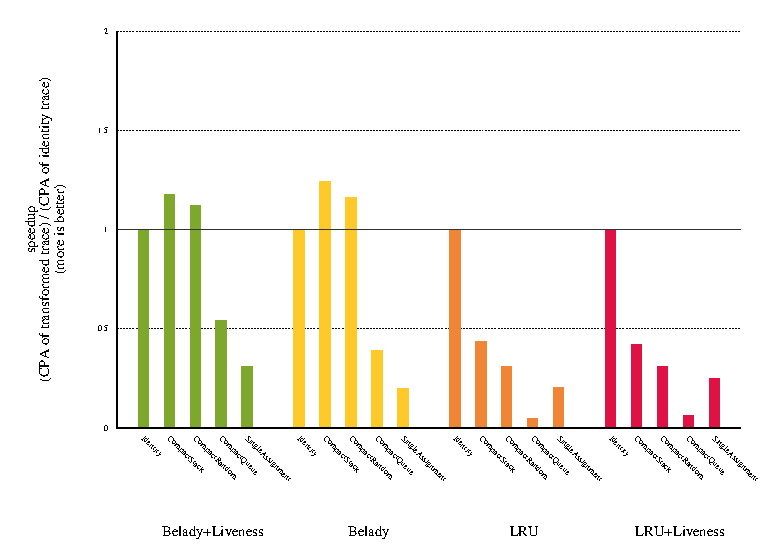
\includegraphics[width=\textwidth]{figs/plots/speedup-richards.eps}
    \subcaption{Speedup}
  \end{subfigure}%
  \begin{subfigure}[b]{0.5\textwidth}%
    \includegraphics[width=\textwidth]{figs/plots/compaction-richards.eps}
    \subcaption{Compaction}
  \end{subfigure}%
  \caption{Speedup \& Compaction: richards}
  \label{fig:speedup-compaction-richards}
\end{figure}

\begin{table}[!ht]
  \centering
  \begin{tabular}{lrrrr}
    \hline
    Benchmark & Count & Average & Minimum & Maximum\\
    \hline
    \csvreader[late after line=\\]{figs/statistical-analysis-data/prepared-address-accesses.csv}
    {1=\colbmk, 2=\colcount, 3=\colmean, 4=\colstd, 5=\colvar, 6=\colmin, 7=\colmax, 8=\colpera,
     9=\colperb, 10=\colperc, 11=\colperd, 12=\colpere}
    {\colbmk & \num{\colcount} & \num{\colmean} & \num{\colmin} & \num{\colmax}}
    \hline
  \end{tabular}
  \\~\\
  \begin{tabular}{lrrrrr}
    \hline
    \multirow{2}{*}{Benchmark} & \multicolumn{5}{c}{Percentile} \\
     & 5\% & 25\% & 50\% & 75\% & 95\% \\
    \hline
    \csvreader[late after line=\\]{figs/statistical-analysis-data/prepared-address-accesses.csv}
    {1=\colbmk, 2=\colcount, 3=\colmean, 4=\colstd, 5=\colvar, 6=\colmin, 7=\colmax, 8=\colpera,
     9=\colperb, 10=\colperc, 11=\colperd, 12=\colpere}
    {\colbmk & \num{\colpera} & \num{\colperb} & \num{\colperc} & \num{\colperd} & \num{\colpere}}
    \hline
  \end{tabular}
  \caption{Metric: Accesses}
  \label{tab:metric-accesses-all}
\end{table}

\begin{table}[!ht]
  \centering
  \begin{tabular}{lrrrr}
    \hline
    Benchmark & Count & Average & Minimum & Maximum\\
    \hline
    \csvreader[late after line=\\]{figs/statistical-analysis-data/prepared-access-distances.csv}
    {1=\colbmk, 2=\colcount, 3=\colmean, 4=\colstd, 5=\colvar, 6=\colmin, 7=\colmax, 8=\colpera,
     9=\colperb, 10=\colperc, 11=\colperd, 12=\colpere}
    {\colbmk & \num{\colcount} & \num{\colmean} & \num{\colmin} & \num{\colmax}}
    \hline
  \end{tabular}
  \\~\\
  \begin{tabular}{lrrrrr}
    \hline
    \multirow{2}{*}{Benchmark} & \multicolumn{5}{c}{Percentile} \\
     & 5\% & 25\% & 50\% & 75\% & 95\% \\
    \hline
    \csvreader[late after line=\\]{figs/statistical-analysis-data/prepared-access-distances.csv}
    {1=\colbmk, 2=\colcount, 3=\colmean, 4=\colstd, 5=\colvar, 6=\colmin, 7=\colmax, 8=\colpera,
     9=\colperb, 10=\colperc, 11=\colperd, 12=\colpere}
     {\colbmk & \num{\colpera} & \num{\colperb} & \num{\colperc} & \num{\colperd} & \num{\colpere}}
    \hline
  \end{tabular}
  \caption{Metric: Access Distance}
  \label{tab:metric-access-distance-all}
\end{table}

\begin{table}[!ht]
  \centering
  \begin{tabular}{lrrrr}
    \hline
    Benchmark & Count & Average & Minimum & Maximum\\
    \hline
    \csvreader[late after line=\\]{figs/statistical-analysis-data/prepared-live-addresses.csv}
    {1=\colbmk, 2=\colcount, 3=\colmean, 4=\colstd, 5=\colvar, 6=\colmin, 7=\colmax, 8=\colpera,
     9=\colperb, 10=\colperc, 11=\colperd, 12=\colpere}
     {\colbmk & \num{\colcount} & \num{\colmean} & \num{\colmin} & \num{\colmax}}
    \hline
  \end{tabular}
  \\~\\
  \begin{tabular}{lrrrrr}
    \hline
    \multirow{2}{*}{Benchmark} & \multicolumn{5}{c}{Percentile} \\
     & 5\% & 25\% & 50\% & 75\% & 95\% \\
    \hline
    \csvreader[late after line=\\]{figs/statistical-analysis-data/prepared-live-addresses.csv}
    {1=\colbmk, 2=\colcount, 3=\colmean, 4=\colstd, 5=\colvar, 6=\colmin, 7=\colmax, 8=\colpera,
     9=\colperb, 10=\colperc, 11=\colperd, 12=\colpere}
    {\colbmk & \num{\colpera} & \num{\colperb} & \num{\colperc} & \num{\colperd} & \num{\colpere}}
    \hline
  \end{tabular}
  \caption{Metric: Overlapping Liveness}
  \label{tab:metric-overlapping-liveness-all}
\end{table}

\begin{table}[!ht]
  \centering
  \begin{tabular}{lrrrrrr}
    \hline
    Benchmark & Count & Average & Minimum & Maximum\\
    \hline
    \csvreader[late after line=\\]{figs/statistical-analysis-data/prepared-liveness-length.csv}
    {1=\colbmk, 2=\colcount, 3=\colmean, 4=\colstd, 5=\colvar, 6=\colmin, 7=\colmax, 8=\colpera,
     9=\colperb, 10=\colperc, 11=\colperd, 12=\colpere}
    {\colbmk & \num{\colcount} & \num{\colmean} & \num{\colmin} & \num{\colmax}}
    \hline
  \end{tabular}
  \\~\\
  \begin{tabular}{lrrrrr}
    \hline
    \multirow{2}{*}{Benchmark} & \multicolumn{5}{c}{Percentile} \\
     & 5\% & 25\% & 50\% & 75\% & 95\% \\
    \hline
    \csvreader[late after line=\\]{figs/statistical-analysis-data/prepared-liveness-length.csv}
    {1=\colbmk, 2=\colcount, 3=\colmean, 4=\colstd, 5=\colvar, 6=\colmin, 7=\colmax, 8=\colpera, 9=\colperb, 10=\colperc, 11=\colperd, 12=\colpere}
    {\colbmk & \num{\colpera} & \num{\colperb} & \num{\colperc} & \num{\colperd} & \num{\colpere}}
    \hline
  \end{tabular}
  \caption{Metric: Liveness Interval Length}
  \label{tab:metric-liveness-interval-length-all}
\end{table}


